\documentclass[10pt]{article}
\usepackage[margin=0.85in]{geometry}
\usepackage[T1]{fontenc}
\usepackage{amsmath,amssymb,booktabs,graphicx,subcaption,placeins}
\usepackage[colorlinks=true,linkcolor=blue,citecolor=blue,urlcolor=blue]{hyperref}
\usepackage{microtype}
\title{Calibration of VCG Training Loss and PenaltyQAOA Penalty Strength}
\author{}
\date{Completed calibration results, 10 September 2026}
\begin{document}
\maketitle
\section{Calibration of Training Loss and Penalty Strength}
\label{cal:sec}
We conducted two calibration studies before the main algorithm comparison. Study A selected a VCG training loss for preparing the uniform superposition of feasible states. Study B selected a rule for setting the shared penalty coefficient in standard PenaltyQAOA. Study B did not use trained VCGs and did not execute PC-QAOA. The studies used separate instance sets and selection criteria. The calibration COPs are reserved from the subsequent algorithm comparison.

\subsection{Study A: VCG Loss Selection}
\label{cal:a}
\paragraph{Constraint set.}
We generated 50 constraints on support sizes $k\in\{4,5,6,7,8\}$, with ten constraints per size and two or three per family within each size. The family totals were 13 positive weighted inequalities, 13 mixed-sign inequalities, 12 weighted equalities, and 12 quadratic inequalities. For positive weighted inequalities, coefficients were integers in $\{1,\ldots,5\}$. If $S$ denotes their sum, the right-hand side was sampled uniformly from the integers between $\max(1,\lfloor S/3\rfloor)$ and $\lfloor2S/3\rfloor$, inclusive. Quadratic inequalities used dense upper-triangular coefficient arrays, including diagonal terms, with coefficients in $\{1,2,3\}$ and the same capacity rule applied to the coefficient sum. Diagonal terms satisfy $x_i^2=x_i$ on binary inputs.

Mixed-sign inequalities used coefficient magnitudes in $\{1,\ldots,5\}$ and required both signs. Writing $a$ and $b$ for the minimum and maximum attainable left-hand-side values, the integer right-hand side was drawn from $[a+\lfloor(b-a)/3\rfloor,\,a+\lfloor2(b-a)/3\rfloor]$. Weighted equalities used positive coefficients in $\{1,\ldots,5\}$ and an attainable right-hand side in the positive-weight capacity range. We rejected empty and fully feasible sets, repeated feasible masks at the same support size, and cases supported by the existing exact-preparation routines, including singleton sets and unions of complete Hamming-weight sectors. The accepted feasible fractions (the total amount of bitstrings feasible out of all $2^k$ bitstrings) ranged from $0.078125$ to $0.90625$ (Fig.~\ref{cal:a-data}).

\begin{figure}[tb]
\centering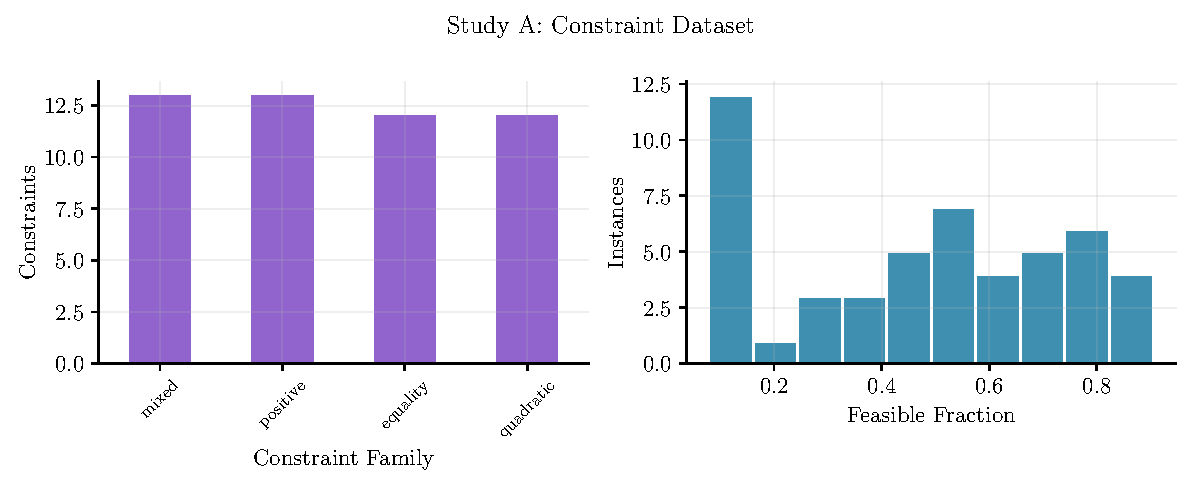
\includegraphics[width=0.88\linewidth]{figures/a_dataset.pdf}
\caption{Study A constraint composition and feasible fractions. A feasible fraction is the number of satisfying bitstrings divided by $2^k$.}
\label{cal:a-data}
\end{figure}

\paragraph{Loss functions.}
For feasible set $\mathcal F$, the target state and evaluation metrics were
\begin{align}
|u_{\mathcal F}\rangle &= |\mathcal F|^{-1/2}\sum_{x\in\mathcal F}|x\rangle,\\
P_{\mathcal F}(\theta)&=\sum_{x\in\mathcal F}|\langle x|\psi_\theta\rangle|^2,\qquad
F(\theta)=|\langle u_{\mathcal F}|\psi_\theta\rangle|^2,\\
F_{\mathrm{cond}}(\theta)&=F(\theta)/P_{\mathcal F}(\theta).
\end{align}


We compared five candidate loss functions, which had the form:
\begin{align}
L_{\mathrm{feas}}&=1-2P_{\mathcal F}, & L_{\mathrm{fid}}&=1-F,\\
L_\lambda&=(1-P_{\mathcal F})+\lambda(1-F_{\mathrm{cond}}),
&&\lambda\in\{0.5,1,2\}.
\end{align}
Every loss was applied to every constraint, giving 250 complete VCG training tasks ($5$ losses $\times 50$ constraints). Each task used one complete training seed and the restart budgets in Table~\ref{cal:budgets}. Initialization seeds were matched across losses for each constraint and depth to compare performance fairly. The inherited optimized angles could differ between losses.

\begin{table}[tb]
\centering
\caption{Training budgets. A restart runs the full stated number of Adam steps. Early stopping in Study A occurs between depths, not within a restart.}
\label{cal:budgets}
\begin{tabular}{lcc}
\toprule
Setting & Study A & Study B\\
\midrule
Standard-QAOA warm-up & $p=1$, $5\times150$ steps & None\\
Main angle strategy & ma-QAOA & Standard QAOA\\
Depths & $1$--$8$ & $1$--$5$\\
Restarts per main depth & 20 & 10\\
Adam steps per restart & 200 & 50\\
Learning rate & 0.05 & 0.01\\
Final measurements per depth & Exact state metrics & 10,000 shots\\
\bottomrule
\end{tabular}
\end{table}

\paragraph{Training and retention.}
Training used the same warm-starting procedure we used in the manuscript; we retained the best angles at the end of each layer of ma-QAOA to initialize subsequent layers of optimization. At each depth, the restart with the lowest final value of its assigned training loss was retained. Fidelity was then evaluated for that state. Training stopped if this fidelity reached $0.999$, or after depth eight. The task returned the highest-fidelity state among the retained depth states. Tasks that failed to reach the threshold remained in the analysis. These fidelity-based stopping and return rules replaced the entropy-based rules of the earlier experimental workflow.

\paragraph{Results.}
The selected loss was $L_{\mathrm{fid}}$, which achieved mean fidelity $0.999719$ and reached $F\geq0.999$ on all 50 constraints (Table~\ref{cal:a-results}). Its mean selected depth was $3.18$, compared with $3.42$--$3.62$ for the conditional-fidelity losses. Each conditional-fidelity loss reached the threshold on 49 constraints. Their mean fidelities were also high, and their small differences from $L_{\mathrm{fid}}$ do not establish a broad performance separation. We should choose $L_{\mathrm{fid}}$ for our loss function.

\begin{table}[tb]
\centering\small
\caption{Study A results across all 50 constraints per loss. Depth columns report the mean selected depth and the mean number of evaluated ma-QAOA depths.}
\label{cal:a-results}
\resizebox{\linewidth}{!}{\begin{tabular}{lrrrrrr}
\toprule
Loss & Mean $F$ & 95\% CI & Mean $P_{\mathcal F}$ & $F\geq0.999$ & Selected $p$ & Evaluated $p$ \\
\midrule
$L_{\mathrm{fid}}$ & 0.999719 & [0.999636, 0.999802] & 0.999849 & 50/50 & 3.18 & 3.18 \\
$L_1$ & 0.999695 & [0.999583, 0.999807] & 0.999837 & 49/50 & 3.42 & 3.44 \\
$L_{0.5}$ & 0.999672 & [0.999550, 0.999794] & 0.999912 & 49/50 & 3.48 & 3.48 \\
$L_2$ & 0.999594 & [0.999427, 0.999761] & 0.999667 & 49/50 & 3.62 & 3.64 \\
$L_{\mathrm{feas}}$ & 0.462554 & [0.385114, 0.539994] & 0.994615 & 2/50 & 1.68 & 7.72 \\
\bottomrule
\end{tabular}
}
\end{table}

The feasibility loss (the one we used in the original manuscript) achieved mean feasible probability $0.994615$, but mean total fidelity was only $0.462554$ and only two constraints reached the fidelity threshold. Its mean selected depth was $1.68$, although it evaluated $7.72$ depths on average. Figure~\ref{cal:a-quality} shows the difference between feasibility and fidelity; Fig.~\ref{cal:a-example} compares the probability distributions for one constraint under two losses. These results support including total fidelity in the training objective when the desired gadget prepares the uniform feasible superposition.

\begin{figure}[tb]
\centering
\begin{subfigure}{0.49\linewidth}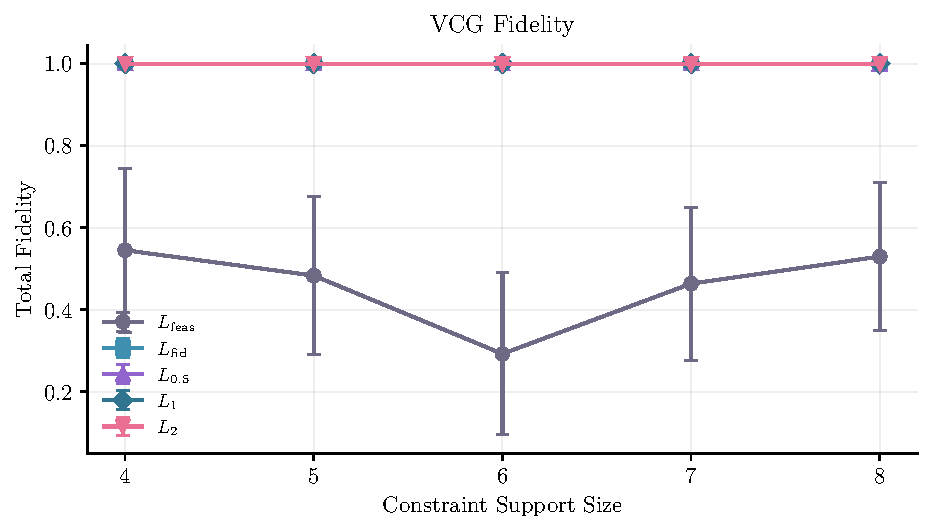
\includegraphics[width=\linewidth]{figures/a_fidelity.pdf}\caption{Returned fidelity by support size.}\end{subfigure}\hfill
\begin{subfigure}{0.49\linewidth}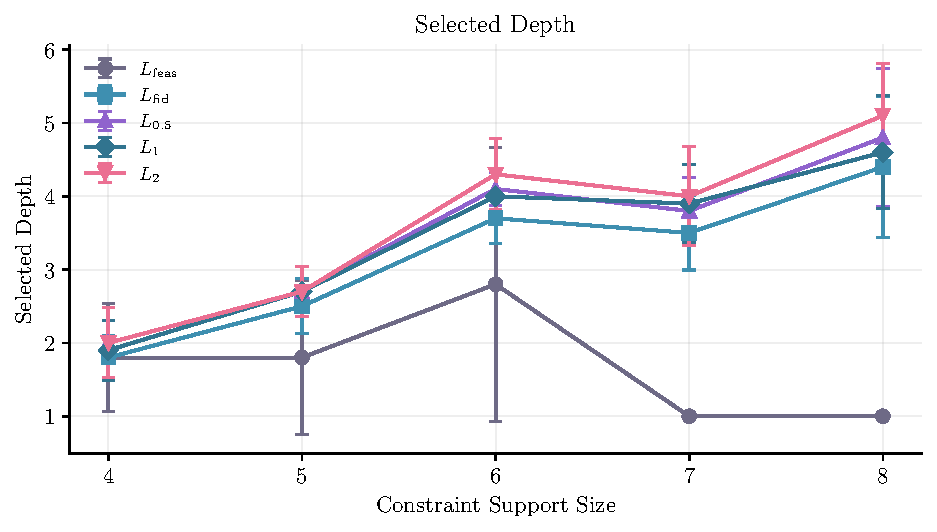
\includegraphics[width=\linewidth]{figures/a_selected_depth.pdf}\caption{Selected depth by support size.}\end{subfigure}
\caption{Study A means and pointwise 95\% confidence intervals across constraints. Each support-size mean contains ten constraints. The selected depth is the depth of the returned gadget, not necessarily the final depth evaluated.}
\label{cal:a-size}
\end{figure}
\begin{figure}[tb]
\centering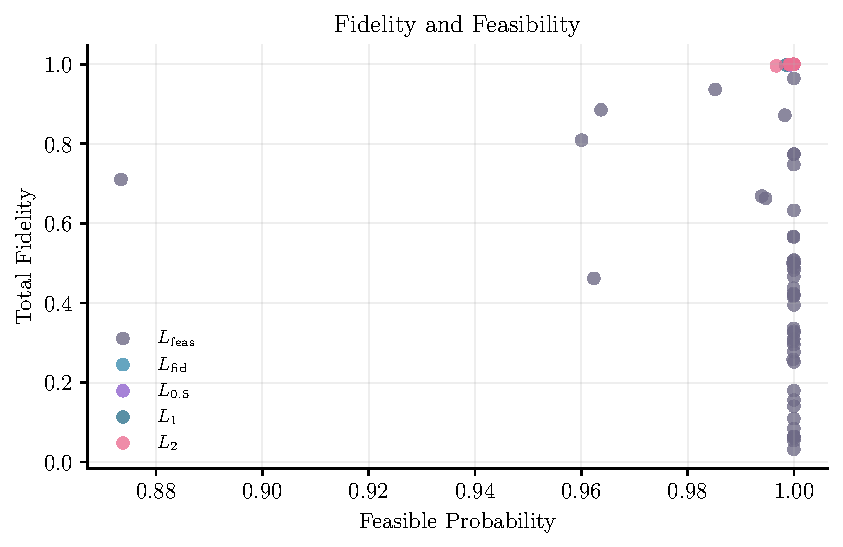
\includegraphics[width=0.7\linewidth]{figures/a_fidelity_feasibility.pdf}
\caption{Returned-state fidelity versus feasible probability. Each point is one constraint--loss task.}
\label{cal:a-quality}
\end{figure}
\begin{figure}[tb]
\centering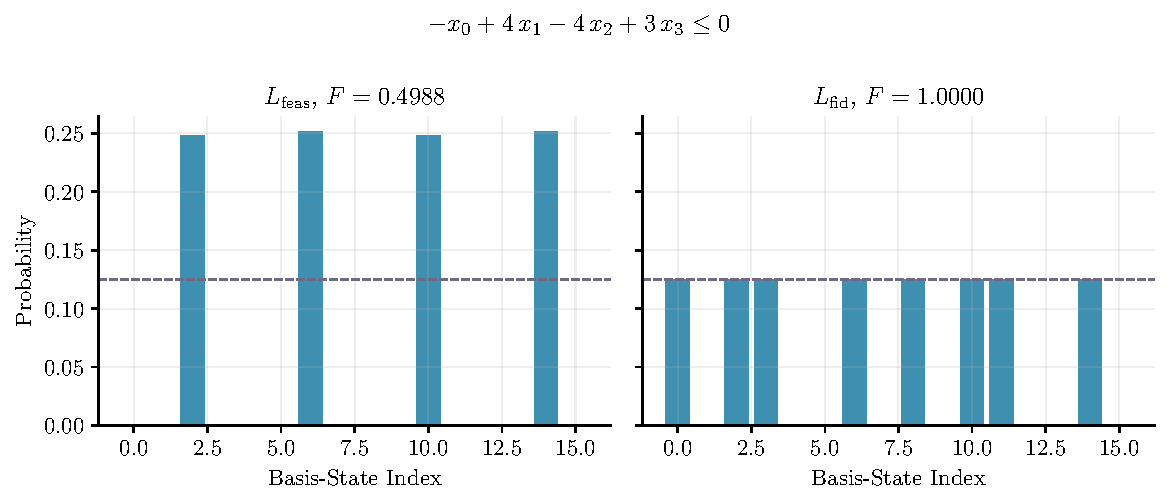
\includegraphics[width=0.92\linewidth]{figures/a_matched_distribution.pdf}
\caption{Returned probability distributions for the same mixed-sign constraint trained with $L_{\mathrm{feas}}$ and $L_{\mathrm{fid}}$. Blue denotes feasible states and rose denotes infeasible states (note how there is no rose!). The dashed line is $1/|\mathcal F|$, the target probability on each feasible state. (Note how bad $L_\mathrm{feas}$ performs compared to $L_\mathrm{fid}$).}
\label{cal:a-example}
\end{figure}
\FloatBarrier

\subsection{Study B: Penalty-Rule Selection}
\label{cal:b}
The goal of this study is to determine the best way to select the penalty parameter $\delta$ used in PenaltyQAOA. 

\paragraph{Calibration problems.}
We generated 20 fresh COPs with decision sizes $n\in\{4,5,6,7,8\}$. Each size contributed two problems with disjoint constraint supports and two with overlapping supports. Across the 50 constraint occurrences, there were 12 cardinality, 10 knapsack, nine quadratic-knapsack, eight flow, six independent-set, and five assignment constraints. The constraints used in this experiment were different from those generated in the VCG training experiment.

Each objective was generated independently as an upper-triangular QUBO with integer coefficients from $-5$ through $4$. The COPs were checked for feasibility and repeated constraint collections were rejected. Joint feasible fractions ranged from $0.0625$ to $0.75$ (Fig.~\ref{cal:b-data}). The complete dataset was saved before training.

\begin{figure}[tb]
\centering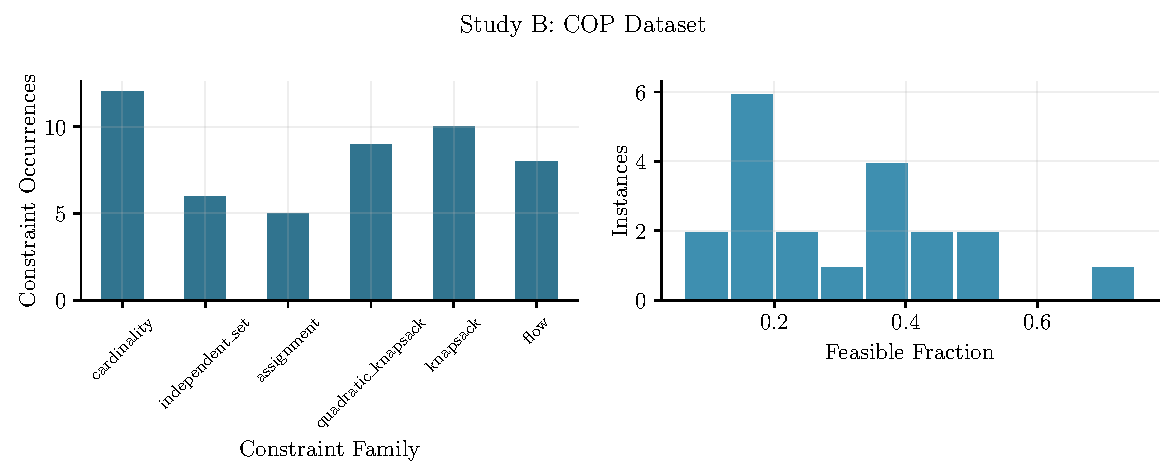
\includegraphics[width=0.88\linewidth]{figures/b_dataset.pdf}
\caption{Study B constraint occurrences and joint feasible fractions. Each feasible fraction counts decision strings satisfying all constraints simultaneously, divided by $2^n$.}
\label{cal:b-data}
\end{figure}

\paragraph{Five penalty rules.}
Write the objective with each coefficient counted once:
\begin{equation}
f(x)=\sum_i q_i x_i+\sum_{i<j}q_{ij}x_ix_j.
\end{equation}
For $i\ne j$, define $c_{ij}=q_{\min(i,j),\max(i,j)}$. Let $q_t$ range over the linear and pairwise coefficients, and set
\begin{equation}
L_Q=\sum_t\min(0,q_t),\qquad U_Q=\sum_t\max(0,q_t).
\end{equation}
The five candidates were
\begin{align}
\delta_{\mathrm{range}}&=U_Q-L_Q+1,\label{cal:range}\\
\delta_{\mathrm{feasible}}&=f(\bar x)-L_Q+1,\\
\delta_{\mathrm{VL}}&=1+\max_i\left\{q_i+\sum_{j\ne i}\max(c_{ij},0),\;-q_i-\sum_{j\ne i}\min(c_{ij},0)\right\},\\
\delta_{\mathrm{local}}&=1+\max_i\left(|q_i|+\sum_{j\ne i}|c_{ij}|\right),\\
\delta_{\mathrm{max}}&=1+\max_t|q_t|.
\end{align}
For each of the 20 COPs, we tested all five $\delta$ options, leading to $100$ total optimized COPs. 

The feasible point $\bar x$ was the first feasible string encountered in a seeded random ordering of decision strings, searched without replacement. No objective values or optimal-solution labels entered that search. The objective was evaluated after the point was chosen. The search required a mean of $3.2$ feasibility checks, with a maximum of 11; its measured mean runtime was approximately $0.149$ ms on this machine. This search is inexpensive for the calibration sizes, but its enumeration-based implementation is not a scalable feasibility algorithm.

The rules $\delta_{\mathrm{range}}$ and $\delta_{\mathrm{feasible}}$ are sufficient for the implemented integer squared-residual encoding. To see this, write the penalized energy as $f(x)+\delta\sum_j r_j(x,s_j)^2$. For an infeasible decision string, its minimum residual sum over slack assignments is at least one. With $\delta_{\mathrm{feasible}}$, its energy is therefore at least $L_Q+\delta_{\mathrm{feasible}}=f(\bar x)+1$, above the energy of a feasible point with valid slack. The bound for $\delta_{\mathrm{range}}$ follows by replacing $f(\bar x)$ with its upper bound $U_Q$. These guarantees concern global energy minima, not the success probability of finite-depth QAOA.

The signed local rule $\delta_{\mathrm{VL}}$ uses the objective-change calculation of Verma and Lewis~\cite{cal:verma}, with an added unit margin. The rules $\delta_{\mathrm{VL}}$, $\delta_{\mathrm{local}}$ and $\delta_{\mathrm{max}}$ are heuristics for the general overlapping constraints considered here. A one-bit objective-change bound alone does not prove that arbitrary infeasible assignments can be repaired with a sufficient decrease in penalty. The sufficient-bound reasoning is consistent with the exact-penalty framework discussed by Diez Garc\'ia et al.~\cite{cal:garcia}; their solver experiments do not establish QAOA performance for these instances.

\paragraph{Optimization and measurements.}
We optimized using standard QAOA with the hyperparameters in Table~\ref{cal:budgets}, following the same warm-starting procedure in the manuscript once again. At each depth, the restart with the lowest final penalized expectation was retained. Final performance was determined by calculating $P(\mathrm{opt})$ from $10{,}000$ measurement shots. 

\paragraph{Results and selection.}
$\delta_{\mathrm{range}}$ achieved the highest mean sampled $P(\mathrm{opt})$, $12.3775\%$, followed by $\delta_{\mathrm{max}}$ at $11.2840\%$ (Table~\ref{cal:b-results}). The ordering of the mean exact probabilities was the same. We should therefore select $\delta_{\mathrm{range}}$ in Eq.~\eqref{cal:range} for the subsequent penalty-based experiments when we do the full PC-QAOA vs. PenaltyQAOA experiment. Figure~\ref{cal:b-methods} reports the final-depth means and the full depth progression.

\begin{table}[tb]
\centering\small
\caption{Study B results at depth five of QAOA, with 20 COPs per method. Probabilities and interval bounds are percentages.}
\label{cal:b-results}
\resizebox{\linewidth}{!}{\begin{tabular}{lrrrr}
\toprule
Method & Sampled $P(\mathrm{opt})$ & 95\% CI & Exact $P(\mathrm{opt})$ & Sampled $P(\mathcal F)$ \\
\midrule
$\delta_{\mathrm{range}}$ & 12.377 & [1.418, 23.337] & 12.403 & 46.127 \\
$\delta_{\mathrm{max}}$ & 11.284 & [2.018, 20.550] & 11.329 & 43.681 \\
$\delta_{\mathrm{VL}}$ & 10.920 & [2.050, 19.790] & 10.856 & 46.550 \\
$\delta_{\mathrm{local}}$ & 10.736 & [1.265, 20.206] & 10.827 & 44.846 \\
$\delta_{\mathrm{feasible}}$ & 9.878 & [0.550, 19.207] & 9.783 & 45.449 \\
\bottomrule
\end{tabular}
}
\end{table}
\begin{figure}[tb]
\centering
\begin{subfigure}{0.49\linewidth}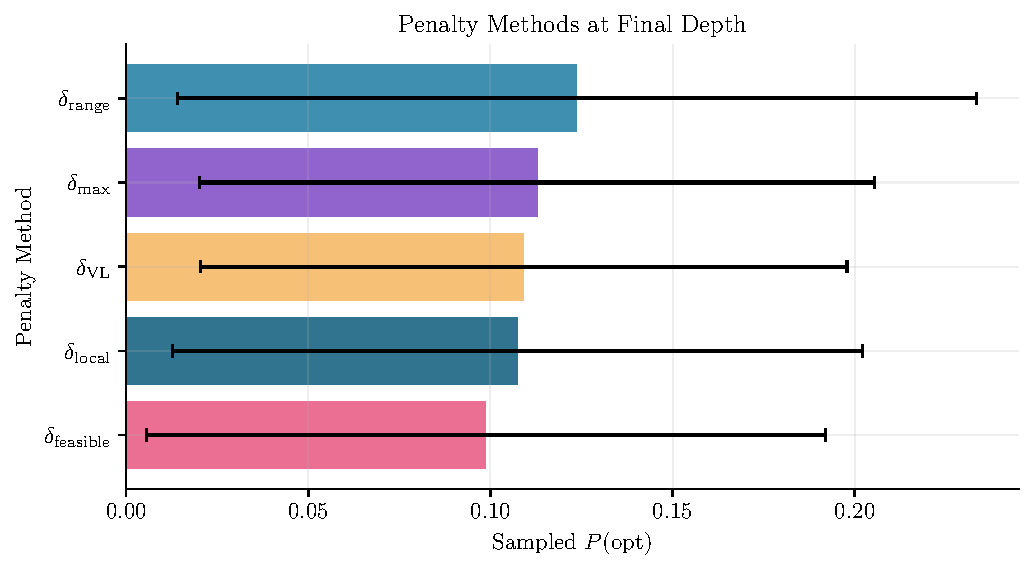
\includegraphics[width=\linewidth]{figures/b_methods.pdf}\caption{Final-depth method comparison.}\end{subfigure}\hfill
\begin{subfigure}{0.49\linewidth}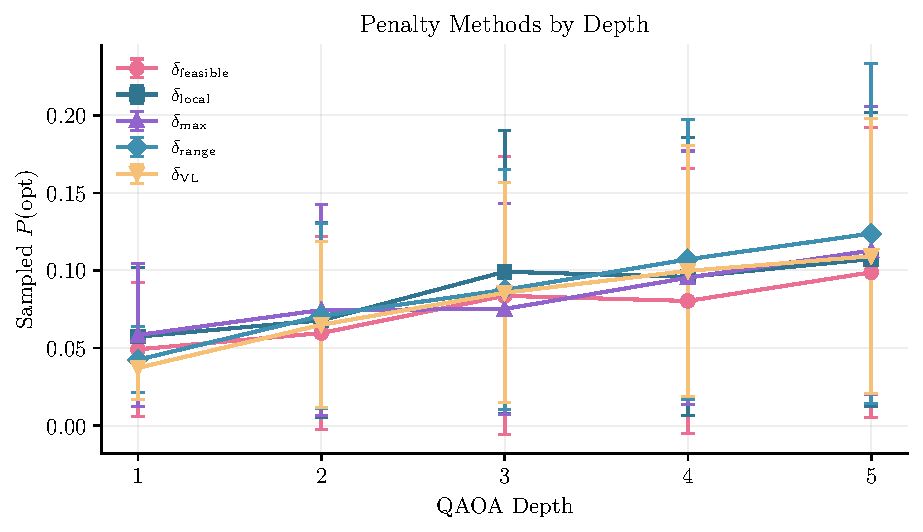
\includegraphics[width=\linewidth]{figures/b_depth_methods.pdf}\caption{Depth progression.}\end{subfigure}
\caption{Study B mean sampled optimal-solution probabilities and pointwise 95\% confidence intervals across 20 COPs. These intervals estimate uncertainty in each method's mean; they are not paired intervals for differences between methods.}
\label{cal:b-methods}
\end{figure}


Performance varied strongly with the sampled instances. For $\delta_{\mathrm{range}}$, mean $P(\mathrm{opt})$ was $40.588\%$ on the four-variable COPs and $0.615\%$ on the eight-variable COPs (Table~\ref{cal:b-size}). Its mean was $21.116\%$ for disjoint COPs and $3.639\%$ for overlapping COPs. These groups also differ in constraint composition and slack count; the differences cannot be assigned to size or overlap alone. The two four-variable disjoint COPs contributed substantially to the mean advantage of $\delta_{\mathrm{range}}$. $\delta_{\mathrm{range}}$ remained first after removing any single COP, but removing both of those COPs changed the leader to $\delta_{\mathrm{max}}$. That post hoc sensitivity check did not change the selection dataset or criterion.

\begin{table}[tb]
\centering\small
\caption{Mean sampled depth-five $P(\mathrm{opt})$ (percent) by decision size, with four COPs per size. Different methods lead at different sizes.}
\label{cal:b-size}
\begin{tabular}{rrrrrr}
\toprule
$n$ & $\delta_{\mathrm{range}}$ & $\delta_{\mathrm{feasible}}$ & $\delta_{\mathrm{VL}}$ & $\delta_{\mathrm{local}}$ & $\delta_{\mathrm{max}}$ \\
\midrule
4 & 40.587 & 34.025 & 31.677 & 32.903 & 33.428 \\
5 & 11.045 & 3.620 & 11.220 & 10.935 & 14.095 \\
6 & 7.940 & 10.237 & 9.605 & 7.255 & 6.582 \\
7 & 1.700 & 1.020 & 0.860 & 1.710 & 1.650 \\
8 & 0.615 & 0.490 & 1.238 & 0.875 & 0.665 \\
\bottomrule
\end{tabular}

\end{table}

The completed calibration supports $L_{\mathrm{fid}}$ as a direct and effective training objective for the sampled VCG families. It selects $\delta_{\mathrm{range}}$ as the penalty rule with the highest aggregate sampled success probability at depth five. It does not show that this rule is optimal at other depths or for each constraint family.

\FloatBarrier
\appendix
\section{Implementation and Reproducibility}
The two studies used the existing repository generators, constraint parsing, VCG circuits, and PenaltyQAOA implementation through the tuning scripts. Computation used PennyLane 0.43.1 with the \texttt{default.qubit} simulator, JAX/JAXlib 0.6.2, Optax 0.2.5, NumPy 2.2.6, and Python 3.13.13, with 64-bit CPU arithmetic. The dataset seed was 42, the training seed root was 7, and the sampling seed root was 19. Stable hashes of instance and phase identifiers derived the optimization seeds. Penalty-setting identifiers additionally entered the sampling seeds. No complete training-seed replication was performed.

Tasks were grouped by constraint or COP to reuse circuit preparation and compiled functions across conditions. Standard-QAOA penalty circuits combined repeated commuting Pauli terms before compilation while retaining separate numerical objective and penalty weights. The shared angle permits this combination without changing the ideal circuit, apart from irrelevant identity phases. VCG circuits retained the existing ma-QAOA parameter layout. Optimization checkpoints stored angles, Adam state, random state and progress every ten steps and at restart, depth and task boundaries. Files were written atomically with a previous-checkpoint backup.

The default allocation was two workers with six physical CPU cores per worker. Accumulated compile/warm-up time was approximately 10.87 worker-hours for Study A and 0.57 worker-hours for Study B; synchronized optimizer-update time was approximately 10.22 and 14.18 worker-hours, respectively. These totals are sums across tasks, not elapsed wall time, and exclude some I/O and analysis costs. Compilation counters include disposable warm-up calls and overhead on reused functions. The largest recorded worker RSS was approximately 14.54 GiB in Study A and 14.82 GiB in Study B. A worker's RSS is a process high-water mark, not a per-task allocation.

PenaltyQAOA used 4--19 total qubits, including 0--12 slack qubits. Figure~\ref{cal:resources} shows the measured simulation times and qubit counts. The displayed PC-QAOA slack counts are computed partitions only; no PC-QAOA simulation is included.

\begin{figure}[tb]
\centering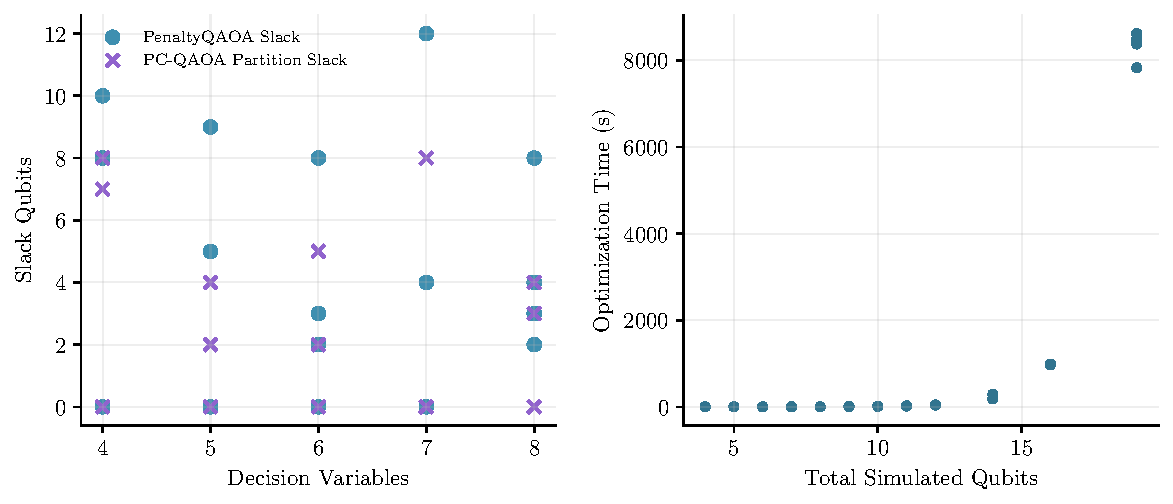
\includegraphics[width=0.9\linewidth]{figures/b_qubits_runtime.pdf}
\caption{Decision/slack counts and recorded PenaltyQAOA optimizer-update times. Each runtime point is a completed instance--method task across depths one through five. The PC-QAOA points represent hypothetical partition slack counts, not measured PC-QAOA execution.}
\label{cal:resources}
\end{figure}

\paragraph{Archived evidence.}
The report's \texttt{data/} directory contains copies of the original run records, manifests and selected-setting records, along with per-task summaries, ranking tables, and paired comparisons. The copied run records preserve source-file hashes, base commit and package versions. Study A and Study B have separate run identifiers because Study B was revised after Study A began. The obsolete multiplier configuration in Study A's run record was not used for the reported Study B results; the separate Study B record specifies the five fixed methods. The report generation record also hashes the analysis source used to produce its tables and figures.

The selected VCG database contains one gadget per calibration constraint trained with $L_{\mathrm{fid}}$. It remains in the original results directory. The report summarizes saved final results and does not modify selections, checkpoints, gadget states or optimizer histories.

\section{Additional Diagnostic Figures}
\begin{figure}[tb]
\centering
\begin{subfigure}{0.49\linewidth}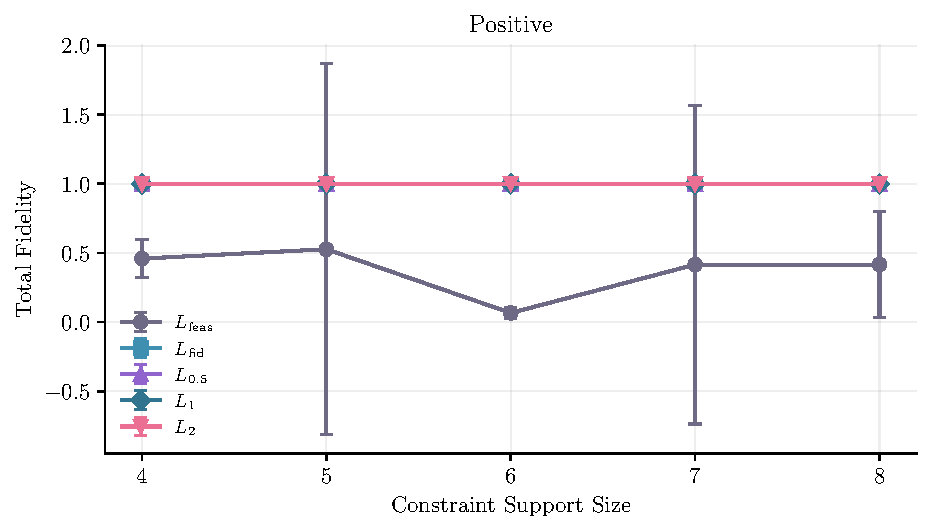
\includegraphics[width=\linewidth]{figures/a_fidelity_positive.pdf}\caption{Positive weighted inequalities.}\end{subfigure}\hfill
\begin{subfigure}{0.49\linewidth}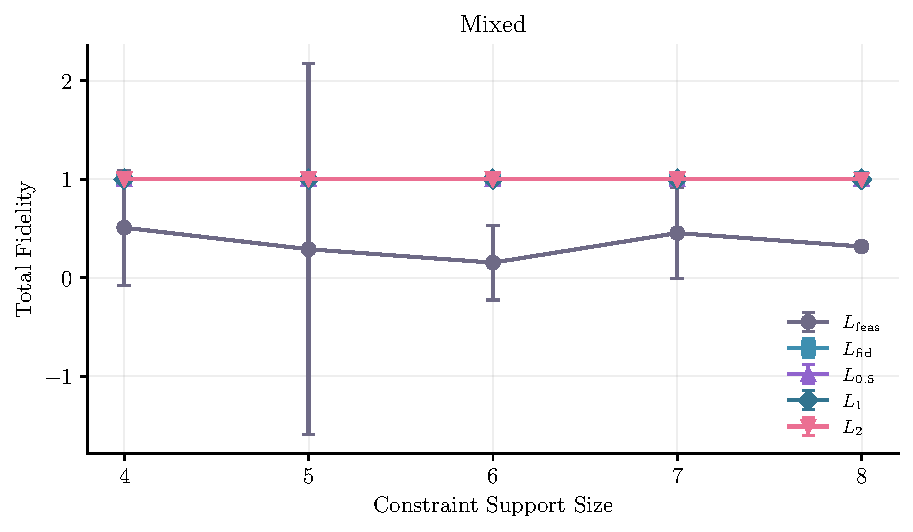
\includegraphics[width=\linewidth]{figures/a_fidelity_mixed.pdf}\caption{Mixed-sign inequalities.}\end{subfigure}\\
\begin{subfigure}{0.49\linewidth}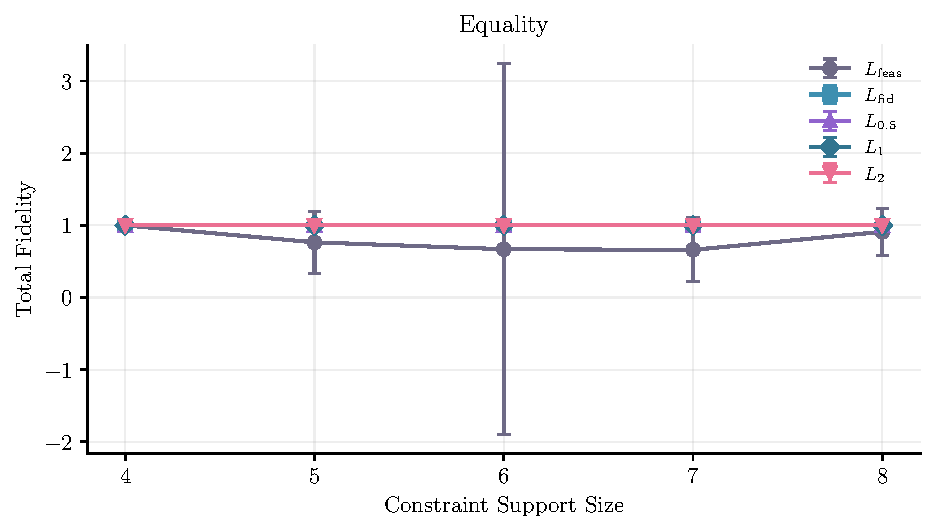
\includegraphics[width=\linewidth]{figures/a_fidelity_equality.pdf}\caption{Weighted equalities.}\end{subfigure}\hfill
\begin{subfigure}{0.49\linewidth}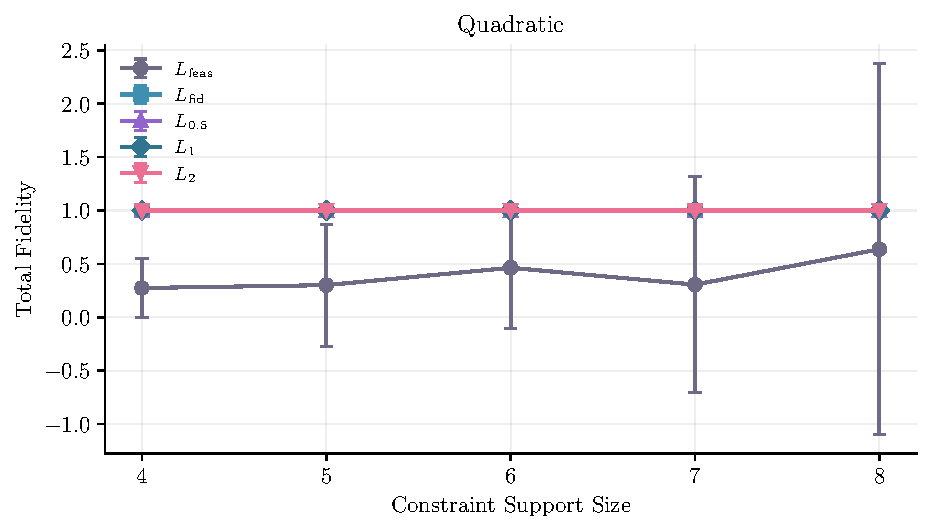
\includegraphics[width=\linewidth]{figures/a_fidelity_quadratic.pdf}\caption{Quadratic inequalities.}\end{subfigure}
\caption{Returned VCG fidelity by family and support size. Each point contains two or three constraints. The pointwise $t$ intervals can be wide or extend beyond physical probability bounds because of the small groups.}
\end{figure}
\begin{figure}[tb]
\centering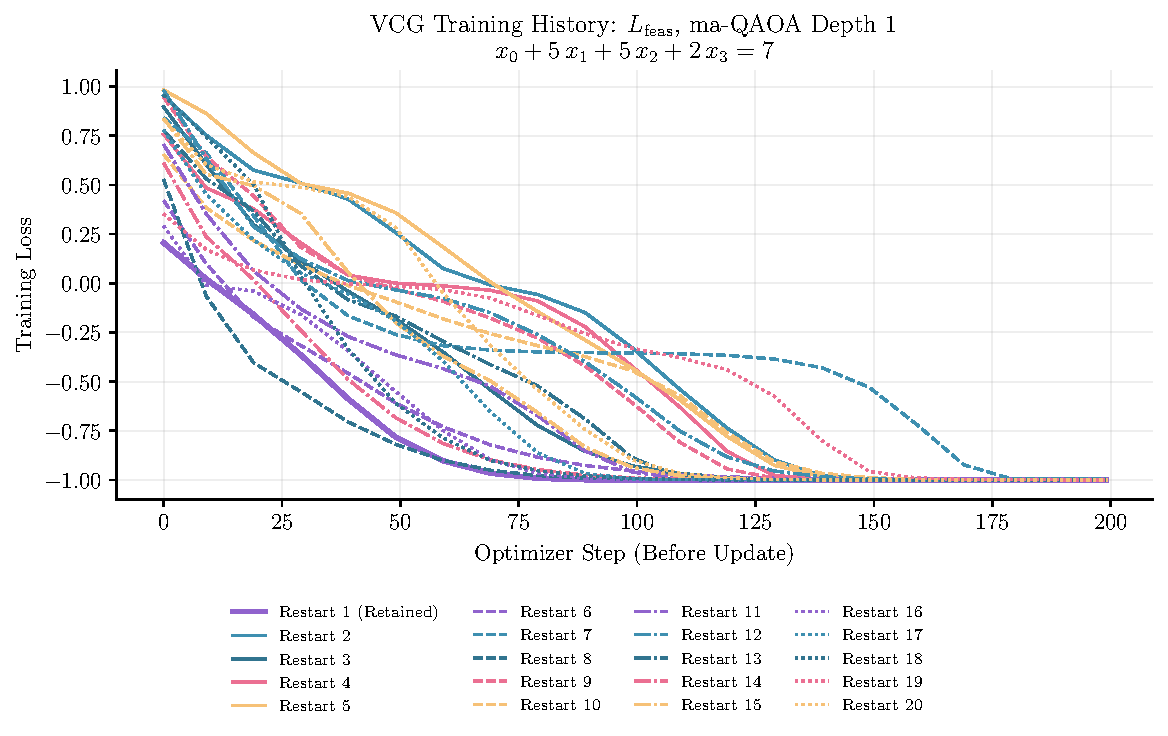
\includegraphics[width=0.8\linewidth]{figures/a_training_history.pdf}
\caption{Example VCG training histories. The title identifies the constraint, loss and depth. Each curve is one restart; the retained restart has the lowest final training loss. The plotted loss is evaluated before the indicated update, whereas restart selection uses the loss after the final update. Loss approaching $-1$ under $L_{\mathrm{feas}}$ indicates feasible probability approaching one, not necessarily uniform-state fidelity approaching one.}
\end{figure}
\begin{figure}[tb]
\centering
\begin{subfigure}{0.49\linewidth}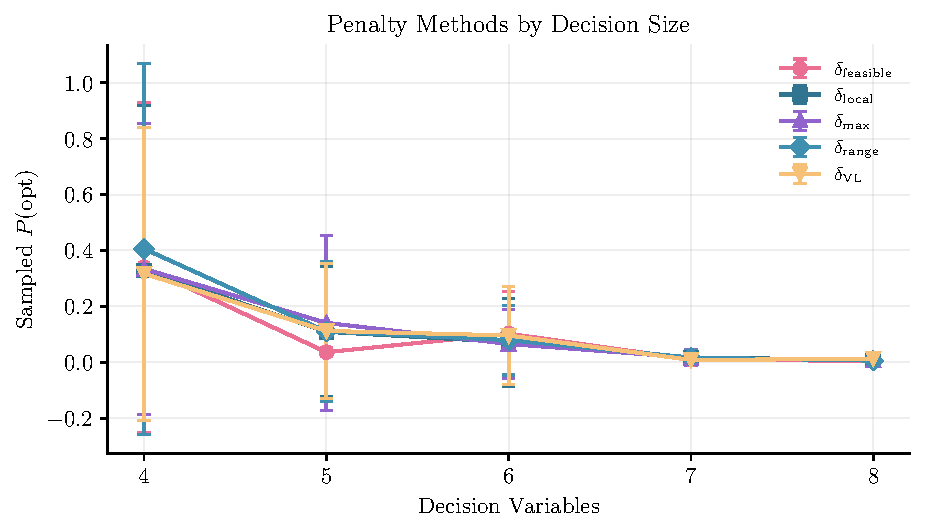
\includegraphics[width=\linewidth]{figures/b_sizes.pdf}\caption{Size dependence.}\end{subfigure}\hfill
\begin{subfigure}{0.49\linewidth}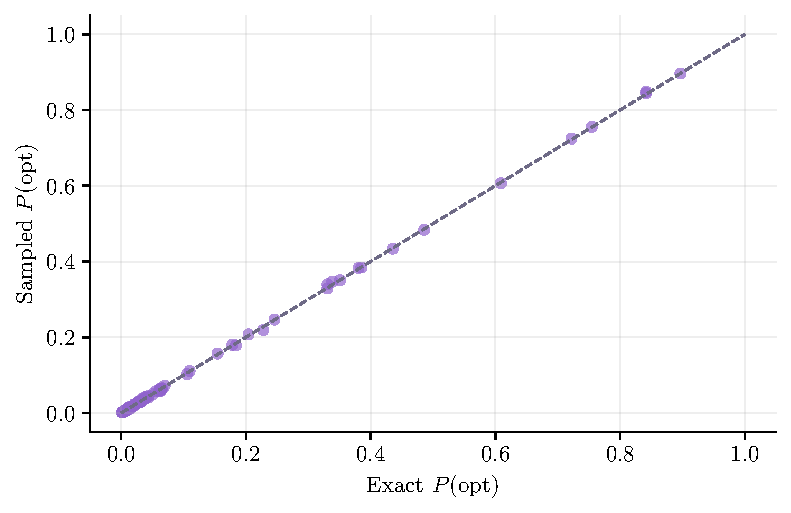
\includegraphics[width=\linewidth]{figures/b_sampled_exact.pdf}\caption{Sampled and exact probabilities.}\end{subfigure}
\caption{Study B diagnostics. Left: means over four COPs per decision size, with pointwise 95\% intervals. Right: exact and sampled depth-five success probabilities for all 100 tasks. The diagonal denotes equality; exact values do not enter penalty selection.}
\end{figure}
\FloatBarrier

\begin{thebibliography}{9}
\bibitem{cal:verma} A. Verma and M. Lewis, ``Penalty and partitioning techniques to improve performance of QUBO solvers,'' \emph{Discrete Optimization} \textbf{44}, 100594 (2022). \href{https://doi.org/10.1016/j.disopt.2020.100594}{doi:10.1016/j.disopt.2020.100594}.
\bibitem{cal:garcia} M. Diez Garc\'ia, M. Ayodele, and A. Moraglio, ``Exact and Sequential Penalty Weights in Quadratic Unconstrained Binary Optimisation with a Digital Annealer,'' \emph{GECCO '22 Companion}, pp. 184--187 (2022). \href{https://doi.org/10.1145/3520304.3528925}{doi:10.1145/3520304.3528925}.
\end{thebibliography}
\end{document}
